\documentclass{llncs}
\usepackage{graphicx}
\graphicspath{ {res/} }
\usepackage{placeins}
\begin{document}
\begin{center}
	
	% Upper part of the page. The '~' is needed because \\
	% only works if a paragraph has started.
	
	\textsc{\LARGE King's College London\\ \small School of Natural and Mathematical Sciences\\ \small Department of Informatics
	}\\[1.5cm]
	
	\textsc{\Large MSc Project Report}\\[0.5cm]
	
	% Title
	\hrule~\\[0.4cm]
	{ \huge \bfseries Smartphone Malware Analysis \\[0.4cm] }
	\hrule~\\[1.5cm]
	
	% Author and supervisor
	\noindent
	\begin{minipage}[t]{0.4\textwidth}
		\begin{flushleft} \large
			\emph{Author:}\\
			Amar Menezes\\(1435460)
		\end{flushleft}
	\end{minipage}%
	\begin{minipage}[t]{0.4\textwidth}
		\begin{flushright} \large
			\emph{Supervisor:} \\
			Dr.~Richard E. Overill
		\end{flushright}
	\end{minipage}
	
	\vfill
	
	% Bottom of the page
	{\large \today}
\end{center}


\begin{abstract} 
	 This report is surveys the two most popular smartphone platforms and the malware landscape associated with these platforms. This is the first part of the final report.
\end{abstract}
\section{Introduction} \label{Intro}
	Traditionally malware authors have targeted personal computers, workstations and servers. Mainly because they were potentially rich stores of sensitive information. Mobile phones on the other hand were mainly used for communication and did not offer much incentive for malware authors. However over the years smartphones and tablets have started replacing personal computers. People now use their smartphones not just to make calls and send messages, but for a host of other applications such as e-commerce transactions, data storage, navigation, socializing etc. Our smartphones now house a lot of our personal and financial information. This provides a huge incentive for malware authors to focus their efforts on attacking smartphones.

	In pre-smartphone era, where each mobile phone vendor used its own proprietary operating system and the phones capabilities itself were limited. Unlike the pre-smartphone era today's smartphones have far greater capabilities from their sophisticated hardware and their constantly improving platforms. The majority of smartphones today run on one of the three platforms which are Android\cite{android-home}, iOS\cite{iOS-home} and Windows Phone\cite{WindowsPhone-home}. As of the 1st quarter of 2015, Android holds a 79.4\% market share, followed by iOS with a 18.3\% and Windows Phone at 3.2\% share \cite{idc-smartphone-marketshare}.
	
	The remainder of this paper is structured as follows. Section \ref{Intro} introduces the problem of smartphone malware and its growth. Section \ref{malware-activities} summarises the malicious activities carried out by malware. Section \ref{capabilities} classifies the various malware types. Section \ref{platforms} summarises the architecture and security models of Android and iOS. Finally Section \ref{malware} describes the attack surface of each platform and malware families.
	
\subsection{Malware attack goals and distribution mechanisms} \label{malware-activities}
Suarez-Tangil et al.\cite{suarez2014evolution} categorised malware based on their attack goal and behaviour, method of distribution and privilege acquisition.\\\\
Attack goals and behaviour are summarised as
\begin{enumerate}
	\item{\textbf{Fraud:} Such as sending SMS/Calling premium numbers or holding device data or functionality ransom.}
	\item{\textbf{Sabotage:} Such as destroying data or rendering the device unusable.}
	\item{\textbf{Theft:} Exfiltration of user information (contact lists, messages, IMEI/IMSI numbers, call/location history etc) and/or user credentials (banking, social accounts, email, corporate accounts)}
	\item{\textbf{SPAM:} Agressive Adware}
	\item{\textbf{Service Misuse:} Such as snooping, spying or tracking of the user by exploiting device sensors. Another example is running a botnet without the users knowledge.}\\
\end{enumerate}
Methods of distribution and infection were categorized as follows
\begin{enumerate}
	\item{\textbf{Market to Device:} An attacker uses an app market to upload his/her malicious application. If markets are not policed for malicious content users are at risk of getting infected.}
	\item{\textbf{App to Device:} In this mode of distribution the attacker uses a vulnerable application to distribute his/her malicious application.}
	\item{\textbf{Web to Device:} This mode of distribution exploits vulnerabilities in web browsers to distribute malicious content.}
	\item{\textbf{SMS to Device:} Malware uses SMS/MMS to distribute malicious payloads. This was a popular strategy targeting the SymbianOS.}
	\item{\textbf{Network to Device:} This strategy exploits platform vulnerabilities or misconfigurations. Distribution uses either Device to Device (D2D) propagation or Cloud to Device (C2D) propagation.}
	\item{\textbf{USB to Device:} Malware infects devices when they are connected to an infected computer via a communication port usually USB.}\\
\end{enumerate}
Privilege acquisition is generally achieved via two methods
\begin{enumerate}
	\item{\textbf{User Manipulation:} An unsuspecting is tricked into granting privileges to malware. User manipulation is achieved via Social Engineering, use of repackaged applications from third-party sources, etc.}
	\item{\textbf{Technical Exploitation:} Here privileges are acquired by exploiting platform vulnerabilities or misconfigurations. Although vulnerabilities differ across platforms, most common attacks include API vulnerabilities, buffer overruns, injection attacks, protocol vulnerabilities etc.}
\end{enumerate}

\subsection{Malware capabilities} \label{capabilities}
Faruki et al. \cite{farukiandroid} categorised malware based on their capabilities within the context of smartphones.
\begin{itemize}
	\item{\textbf{Trojan:} Malicious apps that appear to have a benign purpose to the user, while performing harmful activities without the user being aware. Trojans are typically used in the exfiltration of sensitive data such as user credentials, contacts, messages etc. SMS Trojan families send SMS's to premium rate numbers without the user being aware.}
	\item{\textbf{Backdoors:} This type of malware infects systems exploiting platform weaknesses. Backdoors typically use root exploits to escalate privileges and evade detection.}
	\item{\textbf{Worm:} Malicious apps that create copies of itself which it distributes to other systems via networks and/or removable media.}
	\item{\textbf{Botnets:} These apps compromise the device to create a Bot, which forms part of a network of other such bots called a botnet. Bots are controlled by a Command and Control server and are used for malicious activities ranging from data exfiltration to denial of service attacks.}
	\item{\textbf{Spyware:} These apps perform malicious activites such as monitoring calls, contacts, messages, location, etc. It can also send this data to a remote server controlled by the attacker.}
	\item{\textbf{Adware:} These apps spam the user with unsolicited advertisements and notifications. These can create shortcuts on the home screen, steal bookmarks, and impair effective usage of the device.}
	\item{\textbf{Randsomware:} This type of malware locks the user out of his/her data and demands a ransom to unlock the data.}
\end{itemize}


\section{Smartphone Platforms} \label{platforms}
\subsection{Android}
Android is an open source smartphone operating system being currently developed and maintained by Google Inc. and promoted by the Open Handset Alliance (OHA). Android was originally conceived by Andy Rubin, Chris White, Nick Sears and Rich Miner at Android Inc in October 2003. Android Inc was later acquired by Google Inc in August 2005. The Open Handset Alliance is a consortium of 84 companies led by Google consisting of mobile handset manufactures, software developers, chipset manufactures and a few telecommunication companies \cite{open-hadset-alliance}.

\subsubsection{Ecosystem}
The first Android smartphone was the HTC Dream running Android 1.0 released in September 2008, followed by an upgrade to Android 1.1 in February 2009. From version 1.5 onwards Android releases were codenamed with names of deserts and pastries. The table below summarises the different Android releases and their codenames.
\begin{center} 
\begin{tabular}{|l|c|c|c|r|}       %lcr = allignment of the individual cols
	%| puts a line in between them
	\hline %a line at the top
	Version & Codename & API Level & First Release & Distribution \\
	\hline\hline %puts a line under first row
	1.5 & Cupcake & 1 & April 2009 & \textless 0.1\% \\
	1.6 & Donut & 4 & September 2009 & \textless 0.1\% \\
	2.0.x and 2.1 & Eclair& 5 & October 2009 & \textless 0.1\% \\
	2.2.x & Froyo & 8 & May 2010 & 0.3\% \\
	2.3.x & Gingerbread & 10 & December 2010 & 5.6\%\\
	3.x & Honeycomb & 11 & February 2011 & Unavailable \\
	4.0.x & Ice Cream Sandwich & 15 & October 2011 &  5.1\%\\
	4.1.x, 4.2.x and 4.3.x & Jelly Bean & 16-18 & July 2012 & 37.4\%\\
	4.4.x & KitKat & 19 & October 2013 & 39.2\% \\
	5.x & Lollipop & 21-22 & November 2014 & 12.4\%\\
	\hline %a line at the bottom
\end{tabular}
\end{center}

The ecosystem is not just about the distribution of andriod versions but also comprises of hardware vendors, carriers and developers. Hardware vendors consists of CPU manufacturers, System-On-Chip(SoC) manufacturers and device manufactures.
\begin{itemize}
	\item{\textbf{CPU Manufacturers:} A majority of Android devices run on an ARM architecture based processor due to its low power consumption. ARM Holdings does not manufacture CPUs but licences its technology as intellectual property. The ARMv7 instruction set is common in todays android smartphones.
	In 2011, Google partnered with Intel to support Intel processors on Android. Intel started the Android on Intel Architecture (Android-IA) project to enable Android on Intel processors. Like ARM, MIPS Technologies has licensed its processor architecture designs to other manufacturers. MIPS based proccessors are found in tablets, set-top boxes, media players etc.}
	\item{\textbf{SoC Manufactures:} System-On-Chip are components that include a CPU, GPU, RAM, I/O controllers, baseband processors all included on a single silicon chip. Manufacturing SoCs are more cost effective and power efficient as compared to individual components. The main SoC families are Tegra from nVidia, OMAP from Texas Instruments, Exynos from Samsung and Snapdragon from Qualcomm.}
	\item{\textbf{Device Manufactures:} The final handset the consumers purchase is designed and built by device manufacturing companies. Some well known companies include Samsung, LG, Motorola, HTC and Sony. Device manufactuers tend to customize the Android framework to differentiate themselves from the competition. However these customizations could lead to vulnerabilities in the Android framework. Since the Android framework is licenced under the Apache 2.0 Licence, modified binaries can be redistributed without releasing the source code.}
\end{itemize}

Carriers provide voice and data services to smartphone customers. Some carriers also partner with device manufacturers to provide phone deals to customers. Carrier deals customize the phones firmware before being made available to customers.

Lastly developers form a significant part of the Android ecosystem. Developers contribute to the Android project as well as building applications for the Android platform. Some android enthusiasts also develop custom firmware projects also known as ROMs for different android devices. The most popular of these projects is CyanogenMod \cite{cyanogenmod}.

\subsubsection{Android Architecture}
The Android platform architecture consists of five components. Android applications, the Android framework, the Android Runtime, User-space native code and the Linux kernel.
\begin{figure}[h]
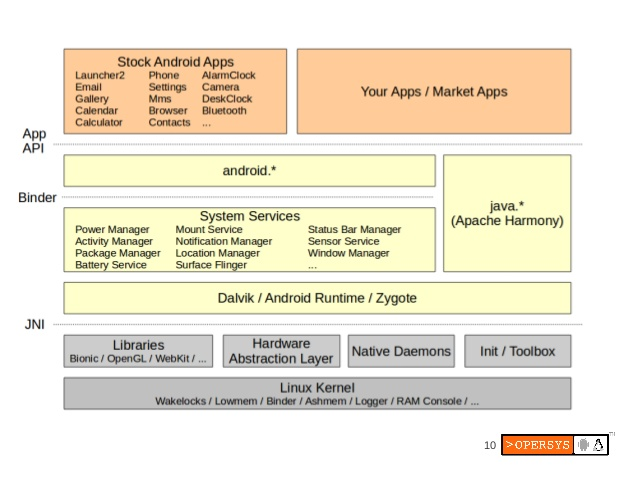
\includegraphics[width=\textwidth]{android_stack}
\centering
\caption{Android platform architecture http://www.slideshare.net/opersys/inside-androids-ui} 
\end{figure}

At the top of the software stack are the Android applications. Application developers use the Android API to build applications that the end user interacts with. Applications found on a device are either system apps which come installed with the stock OS and user installed apps which can be installed from the Google Play Store or other sources.
The Android Framework provides application developers a rich API to access the devices capabilities. The framework allows developers to manage UI interaction, access to media storage, access to device peripherals such as the baseband controller, camera, GPS, wifi controllers, inter process communication, etc.
The Android Framework and Android applications are developed in Java. Applications are compiled into Dalvik Executables (or dex files) which are then interpreted by the DalvikVM. The DalvikVM is a register based virtual machine that executes applications written for Android. The DalvikVM forms an integral part of the Android Runtime and provides a layer of abstraction to the underlying operating system. Android 4.4 (KitKat) introduced a new runtime called Android Run Time (ART) as an experimental alternative. Unlike Dalvik which used Just-In-Time compilers to convert dex bytecode into native code, ART uses Ahead-Of-Time compilers to compile the application into native code upon their installation. In Android 5.0 ART replaced Dalvik as the sole Android runtime.
In addition to the Android Framework, developers can access system services (eg. dhcpd, wpa\_supplicant,etc) and system libraries(eg bionic libc, WebKit, OpenSSL, etc) via user-space native code components. These components allow access to services and libraries that talk directly to the Linux kernel and avoid the overhead of the Android Runtime. Low-level native code operations are employed when application performance is paramount.
The final component of the Android stack is the Linux kernel. The kernel has been modified to operate smartphone hardware. Kernel drivers control device peripherals, network components, process management and file system access. Some of the android specific kernel drivers are wakelocks for power management, ashmem for anonymous shared memory, alarms, paranoid networking and Binder. Paranoid networking and Binder are important from a security perspective as the former restricts access to network sockets to applications based on their permission set and the latter implements Inter Process Communication (IPC) and an associated security mechanism. 

\FloatBarrier
\subsection{Application structure and components}
Android applications are distributed in via APK (Android PacKage) files. An apk is an zip archive with of several files and folders. A typical android application has a folder structure as shown in \ref{apk_struct}
\begin{figure}[h] \label{apk_struct}
	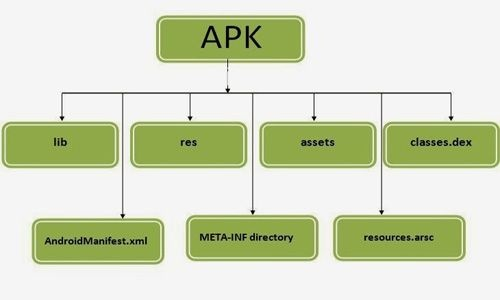
\includegraphics[width=\textwidth]{apk_structure}
	\centering
	\caption{Android package structure http://www.quora.com/What-is-an-APK-file} 
\end{figure}
\begin{itemize}
	\item{\textbf{AndroidManifest.xml:} This file includes the application meta-data such as package name, minimum and maximum supported API level, permissions requested, libraries used and application components such as Activities, Services, Broadcast Receivers and Content Providers.}
	\item{\textbf{classes.dex:} This file contains the Dalvik bytecode to be executed by the DalvikVM.}
	\item{\textbf{META-INF:} This folder contains the application certificate and a list of files included in the apk along with their SHA-1 hashes.}
	\item{\textbf{lib:} This folder contains native binaries that the application uses. These binaries are stored in sub-folders, created for each supported CPU architecture.}
	\item{\textbf{assets:} This folder contians application assets that can be retrieved by the AssetManager class.}
	\item{\textbf{res:} This folder contains resources that are not compiled into the resources.arsc file. These include icons, images, UI layouts, menus, etc.}
	\item{\textbf{resources.arsc:} This file contains resources that are pre-compiled, for example application strings.}

\end{itemize}

\FloatBarrier
\subsection{Security Model}

\begin{itemize}
 \item{Security features}
 \item{Android application execution}
\end{itemize}

\subsection{iOS}
\begin{itemize}
 \item{Origin}
 \item{Ecosystem}
 \item{Architecture/Software Stack}
 \item{Security Model}
 \item{Security features}
 \item{iOS application execution}
\end{itemize}

\section{Smartphone malware} \label{malware}
\subsection{Android}
\begin{itemize}
\item{Attack vectors}
\item{Known malware families and their capabilities}
\end{itemize}

\subsection{iOS}
\begin{itemize}
\item{Attack vectors}
\item{Known malware families and their capabilities}
\end{itemize}

\section{Malware Analysis Process} \label{process}
\subsection{Overview}
Malware analysis generally follows three steps
\begin{enumerate}
	\item{Detect}
	\item{Analyse}
	\item{Report}
\end{enumerate}

\subsection{Input and Output}
Before we can develop a process we need to define the inputs to the system and the expected output.
\begin{itemize}
	\item{\textbf{Input:} The input to the process would be an Android application package (.apk) that is suspected to be malware.}
	\item{\textbf{Output:} The output from the process would be a report that documents the outcome of the malware analysis.}
\end{itemize}  

\subsection{Proposed Method}
\begin{enumerate}
\item{Utilize online analysis services to analyse the sample. Collect analysis reports.}
\item{Create physical and virtual sandboxes for controlled analysis.}
\item{The Analysis sandbox should be setup with behaviour monitoring tools so as to perform dynamic analysis.}
\item{Analyse information gathered from behaviour monitoring tools to look for malicious activity.}
\item{Decompile the application for static code analysis.}
\item{Generate a report to summarize the analysis and document items of interest.}
\end{enumerate}

\subsection{Implementation}
This sections details the creation of the sandboxes, setup and configuration of behaviour monitoring tools and performing analysis with static analysis tools.

\subsection{Report}
This section describes the report template. The mandatory and optional sections of the report.

\section{Case study} \label{study}
This section applies the proposed method and documents our findings.

\section{Limitations}
\subsection{analysis evasion techniques}
\subsection{detection of colluding apps}
\subsection{Limitations of analysis tools}

\section{Conculsion}

\bibliographystyle{plain}
\bibliography{bibliography}
\end{document}
